% !TEX root = ../main.tex

\chapter{数据集构建与标准化预处理}

\section{实验数据集介绍}
  \subsection{OAI-ZIB 数据集}
    OAI-ZIB数据集是膝关节医学影像研究领域中的“金标准”数据集之一。
    OAI（Osteoarthritis Initiative）是美国的一个长达数年的前瞻性研究项目，旨在识别骨关节炎（Osteoarthritis , OA）的生物标志物。
    它是由Zuse Institute Berlin（ZIB）在OAI原始数据库的基础上，筛选了507例膝关节病例，经过专家手工精细标注而形成的子集。
    该数据集提供了极高空间分辨率的三维解剖信息，具体为 \qty{0.7000}{\milli\metre} $\times$ \qty{0.3646}{\milli\metre} $\times$ \qty{0.3646}{\milli\metre}是开发和验证自动分割、定量软骨分析算法的主流选择。
    \subsubsection{DESS 序列的技术原理}
      OAI-ZIB 数据集的采集主要基于 3D DESS 序列\cite{peterfyOsteoarthritisInitiativeReport2008}。
      这是膝关节扫描中最具代表性的序列之一。
      DESS 序列是一种梯度回波（Gradient Recalled Echo, GRE）技术。
      在 DESS 序列中，由于重复时间（Repetition Time, TR）短于组织的纵向弛豫时间 $T_1$ 和横向弛豫时间 $T_2$，系统在单次激发后无法恢复至初始的热平衡状态。
      在经过连续的射频（Radio Frequency, RF）脉冲诱导，系统最终保持动态平衡，即稳态（Steady State, SS）。
      此时，每一次脉冲都会产生两个截然不同的信号部分。
      \par DESS 的核心在于，在一个TR周期内同时采集两个（或更多）回波信号（$S^+$ 和 $S^-$），通过合并这些信号，可以获得极高的信噪比。
      $S^+$ 信号是在激发脉冲后立即产生的自由感应衰减（Free Induction Decay, FID）信号，其对比度特征主要受 $T_1/T_2^\ast$ 影响，
      具有较高的信噪比（Signal Noise Ratio, SNR），但对 $T_2$ 的对比度相对较弱。
      $S^-$ 信号是由于后续脉冲对之前残余的横向磁化矢量进行回聚形成的回波信号，经过了较长的时间，具有极强的 $T_2$ 权重，对关节积液和软骨的信号非常敏感。
      \par DESS 序列通过以下公式合成最终信号 $S$，既保留了 $S^+$ 的高信噪比，
      又增强了 $S^-$ 的强烈 $T_2$ 对比度，使得软骨呈现中等偏高信号，而滑液呈现极高信号，形成了极其清晰的界面。
      \begin{equation}
        S = \sqrt{S^{+2} + S^{-2}}
      \end{equation}
      \begin{figure}[!htp]
        \centering
        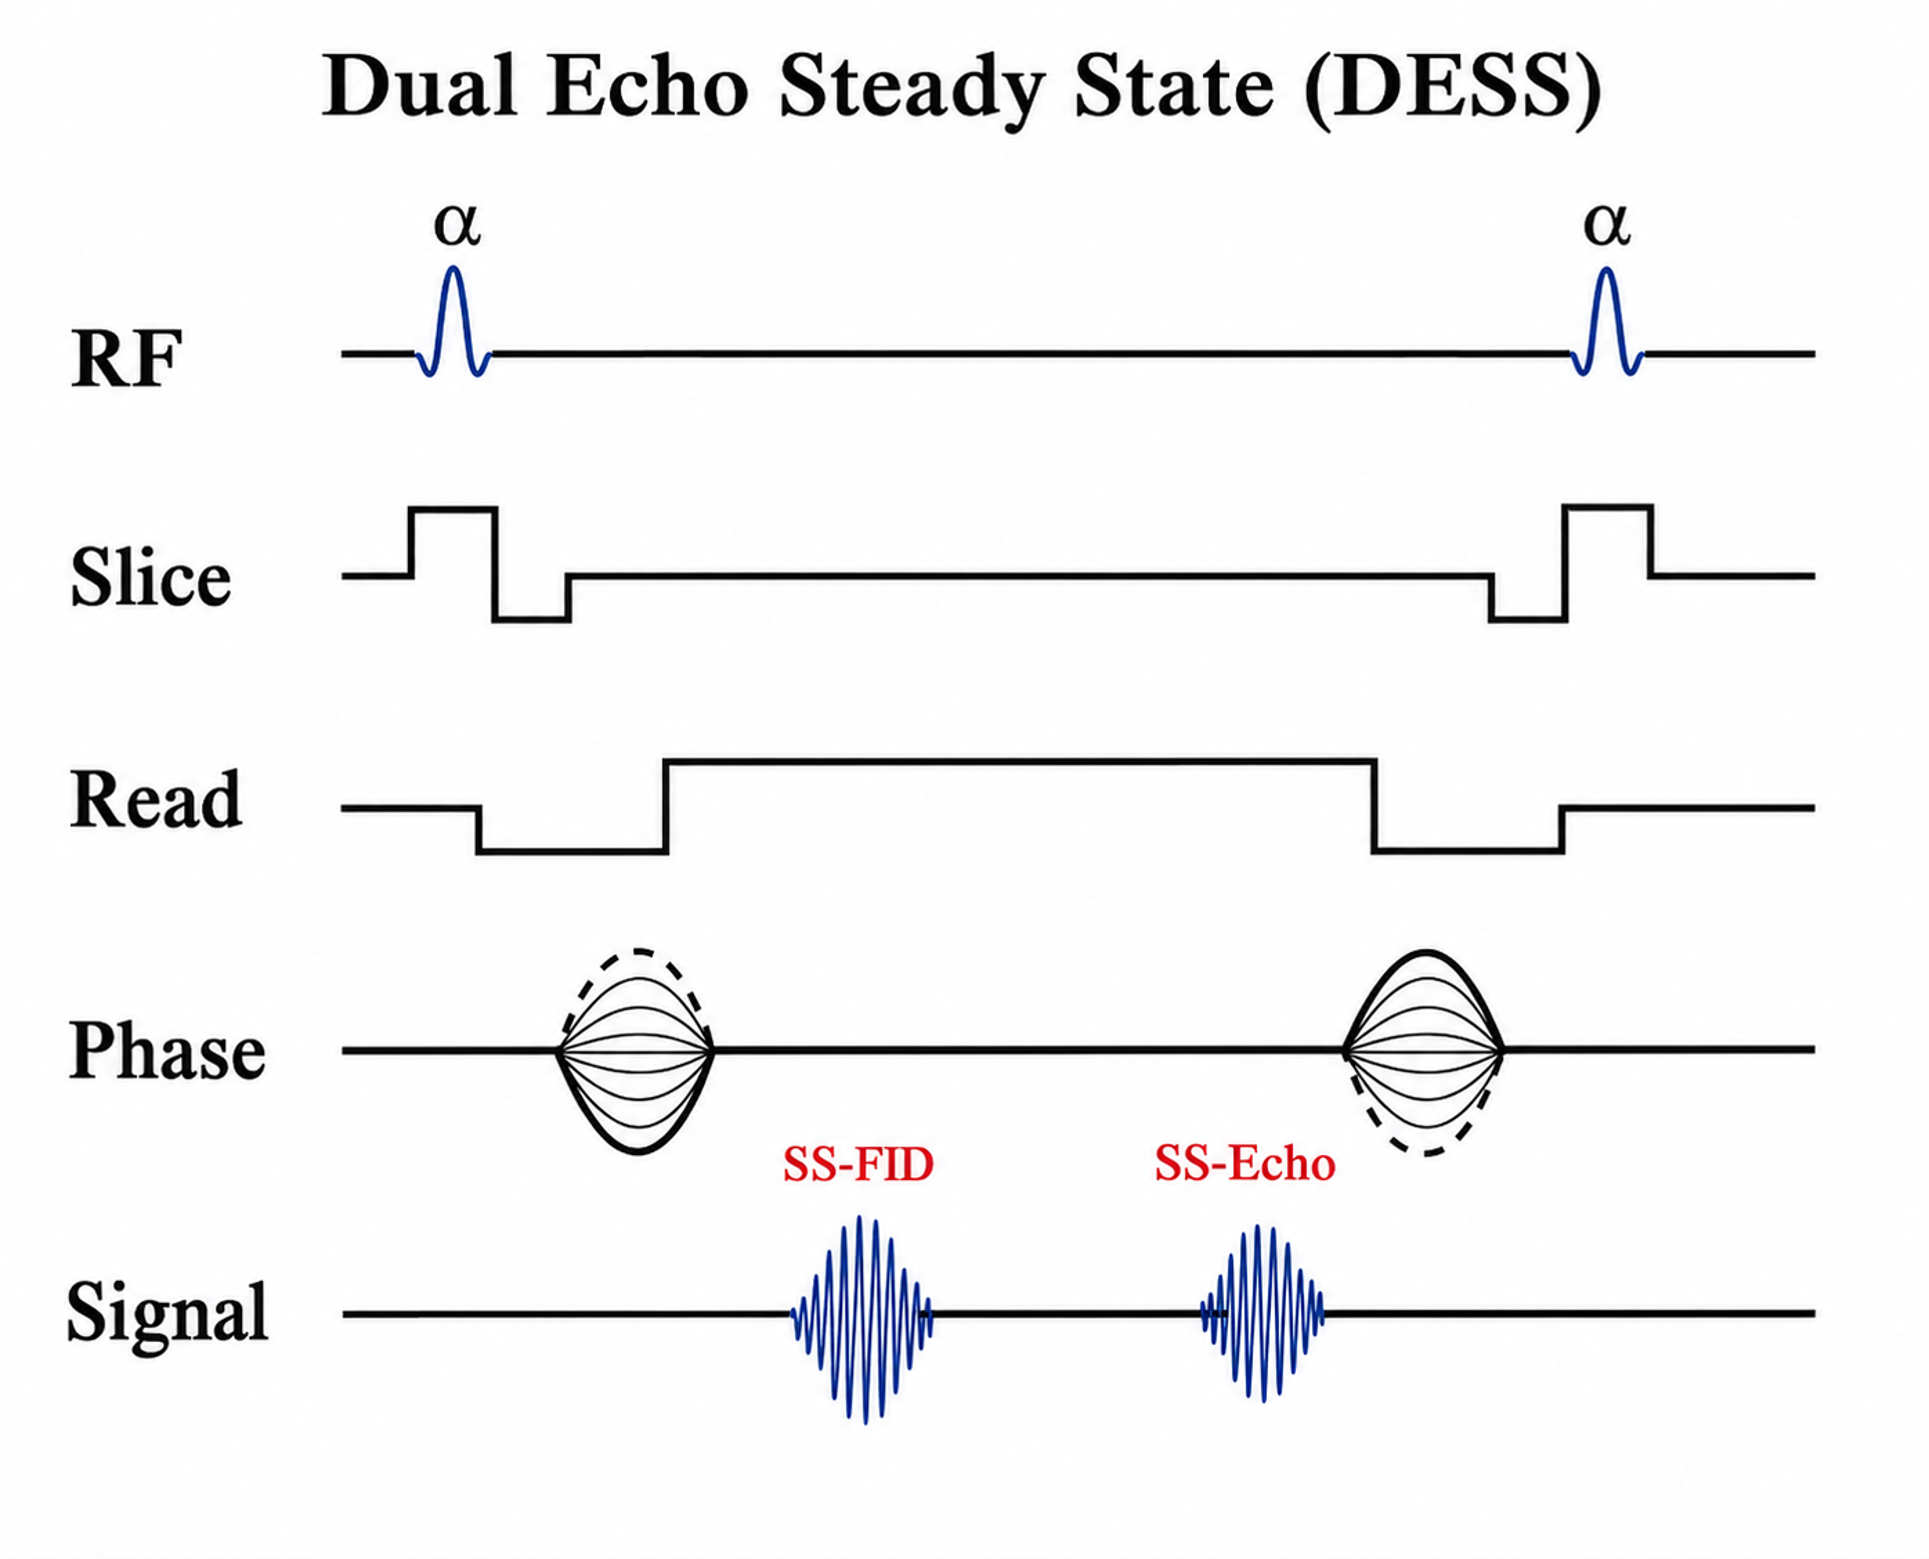
\includegraphics[width=0.8\linewidth]{figures/dess.png}
        \caption{DESS序列示意图}
        \label{fig:dess}
      \end{figure}
    \subsubsection{OAI-ZIB 数据集的分割掩膜与关键参数}
      OAI-ZIB 数据集包含了 507 例受试者的基线期膝关节三维磁共振影像。
      这些影像均采用西门子 3.0T 磁共振扫描仪（Siemens 3.0T Trio scanners）获取，
      扫描序列为矢状面三维双回波稳态（3D Sagittal Double Echo Steady-State, DESS）序列。
      \par 在物理空间参数方面，该数据集具有极高的分辨率配置，为模型提取微小软骨边界提供了充足的像素信息。
      每个三维体积数据（Volume）由 160 张连续的矢状面切片构成，单张切片的矩阵尺寸统一为 384×384 像素。
      其物理体素间距（Voxel Spacing）呈现高度的面内各向同性，具体尺寸为 \qty{0.3645}{\milli\metre} $\times$ \qty{0.3645}{\milli\metre}，层厚（Slice Thickness）为 \qty{0.7}{\milli\metre}。
      此外，在疾病严重程度的分布上，这 507 例数据覆盖了从健康到不同程度的膝关节骨关节炎（OA）患者，并且包含了大量中度至重度的骨关节炎病例。
      这种包含丰富病理形态（如软骨大面积缺损、骨赘增生）的数据分布，使得基于此训练的深度学习网络能够学习到更具鲁棒性和泛化能力的解剖学表征。
      \par 该数据集最核心的价值在于其提供了目前开源领域内最高质量的骨与软骨三维分割掩膜（Ground Truth）。
      OAI-ZIB 的掩膜采用 5 分类标签体系对膝关节主要承重结构进行了像素级映射：
      \begin{itemize}
        \item Label 0：背景区域（Background）
        \item Label 1：股骨（Femoral Bone, FB）
        \item Label 2：股骨软骨（Femoral Cartilage, FC）
        \item Label 3：胫骨（Tibial Bone, TB）
        \item Label 4：胫骨软骨（Tibial Cartilage, TC）
      \end{itemize}
      \par 在标注工艺上，这批数据的金标准并非完全依赖纯人工勾画（纯人工勾画耗时过长且存在较大的阅片者间变异性），
      而是采用了一种“算法生成 + 专家修正”的高效高精度管线。
      首先，研究人员利用三维统计形状模型（Statistical Shape Models, SSMs）结合 2D 与 3D 卷积神经网络（CNNs）进行初始分割，
      随后由经验丰富的影像学专家对网络输出的边界进行极其严格的手动像素级微调与校正。
      \par 这种标注方式使得 OAI-ZIB 的分割掩膜在具有极高解剖学保真度的同时，达到了亚体素级（Sub-voxel）的精度，其准确度与人类专家的观察者间变异度（Inter-observer variability）相当。
      在本研究中，我们将这 507 例高精度的 DESS 序列及标签作为域对抗神经网络（DANN）的源域输入，以指导模型在无标注的 FSE 临床目标域数据中准确寻找到软骨与骨骼的空间拓扑流形。
      \begin{figure}[!htp]
        \centering
        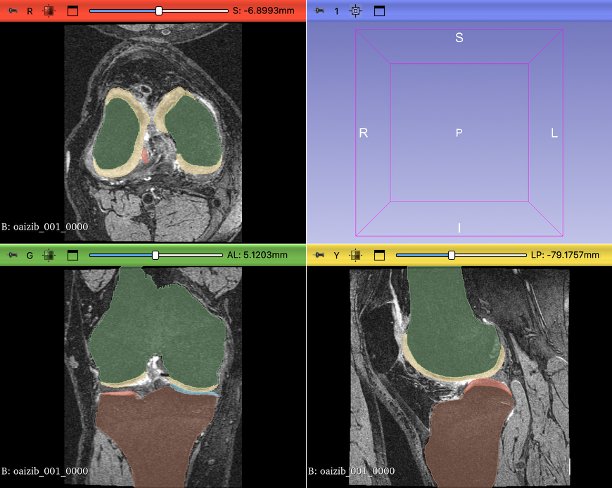
\includegraphics[width=0.8\linewidth]{figures/oaizib.png}
        \caption{OAI-ZIB数据集示例}
        \label{fig:oaizib}
      \end{figure}
  \subsection{孤立前交叉韧带损伤数据集与多发韧带损伤数据集}
    \subsubsection{临床目标域数据分布与无监督痛点}
      本研究的目标域数据来源于真实的骨科与运动医学临床环境，共计收集了665例患者的膝关节磁共振影像。
      在损伤类型分布上，包含500例孤立性前交叉韧带（ACL）撕裂患者，以及165例遭遇高能创伤的多发韧带损伤（MLKI）患者。
      所有影像均采用了带有脂肪抑制技术的快速自旋回波（Fat-suppressed FSE）序列进行采集。
      与作为源域的公开标准化OAI-ZIB数据集不同，这批大量的临床数据完全缺乏由影像科专家提供的像素级解剖结构掩膜。
      这种典型的“有数据、无标签”特征，构成了本研究引入无监督域适应（UDA）框架与自监督超分辨率重建算法的核心驱动力。
      \begin{table}[!hpt]
        \caption{临床目标域数据分布统计}
        \label{tab:clinical_data_distribution}
        \centering
        \begin{tabular}{ccccc} % 五列，居中对齐
          \toprule
          类别 & 性别 & 人数 & 年龄（岁） & 比例（\%） \\
          \midrule
          \multirow{3}{*}{孤立 ACL} 
            & 男性 & 346 & $30.51 \pm 8.94$ & 69.20 \\
            & 女性 & 154 & $33.19 \pm 11.72$ & 30.80 \\
            & 总计 & 500 & $31.33 \pm 9.94$ & 100 \\
          \midrule
          \multirow{3}{*}{多韧带损伤}
            & 男性 & 94 & $35.87 \pm 13.61$ & 56.97 \\
            & 女性 & 71 & $38.75 \pm 12.15$ & 43.03 \\
            & 总计 & 165 & $37.11 \pm 13.04$ & 100 \\
          \bottomrule
        \end{tabular}
      \end{table}
    \subsubsection{代表性测试集的精细化人工标注}
      尽管本研究构建的深度学习管线（如改进型DANN与基于深度图像先验的多视图融合）在网络训练与特征学习阶段能够完全脱离目标域标签运行，
      但为了在模型测试阶段提供具有统计学意义的、严谨客观的性能评估基准（Ground Truth），必须构建一个小规模但高保真的本地测试集。
      \par 为此，本研究在665例目标域数据中，综合考虑了损伤机制、病变严重程度以及影像解剖特征的多样性，严格筛选出具有代表性的30例患者影像。
      针对这30例数据（包含约350个连续二维切片），开展了极其耗时且精细的纯人工标注工作。
      在标注过程中，严格遵循骨与软骨的生理边界，完成了对股骨（Femur）、胫骨（Tibia）以及极易出现视觉断层的关节软骨（Cartilage）的像素级精准勾画。
      \begin{figure}[!htp]
        \centering
        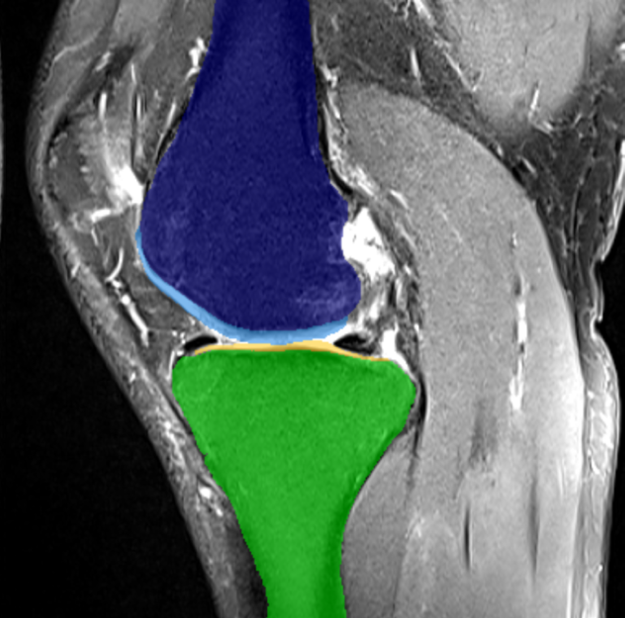
\includegraphics[width=0.5\linewidth]{figures/manual_label.png}
        \caption{精细化人工标注示例}
        \label{fig:manual_label}
      \end{figure}
    \subsubsection{标注数据在研究管线中的定位}
      在整个跨域迁移与网络对抗训练过程中，这30例带有标签的FSE数据被严格隔离，绝不参与任何梯度计算与网络权重的反向传播更新。
      其核心价值在于模型推理阶段：通过计算网络预测掩膜与人工标注掩膜之间的Dice相似系数、平均表面距离（ASD）等空间重叠度量指标，
      有效地量化并验证了DANN模型在克服跨序列域偏移（Domain Shift）上的卓越能力，
      为后续开展大规模骨髓病变（BML）和软骨体积的宏观临床统计奠定了坚实、可信的数据基础。
    \subsubsection{临床数据的伦理审批与患者隐私保护}
      本研究涉及的所有临床目标域数据收集与回顾性分析过程，均已获得上海交通大学附属第六人民医院医学伦理委员会的正式审查与批准（伦理审批编号：2025-KY-295 (K)）。
      所有纳入本研究队列的患者或其法定代理人在接受MRI扫描与临床诊疗前，均已充分知晓研究目的及潜在风险，并签署了书面知情同意书。
      在数据导出与预处理阶段，研究人员已对所有DICOM文件的头信息进行了极其严格的脱敏与去标识化（De-identification）处理，彻底移除了姓名、身份证号等直接隐私数据。
      整个研究的数据管理与使用严格遵循《赫尔辛基宣言》的医学伦理基本原则与患者数据保密规范。
\section{图像预处理流程}
  \subsection{格式的转换与数据清洗}
    在临床医学影像研究中，原始的核磁共振（MRI）数据通常以医学数字成像和通信（Digital Imaging and Communications in Medicine, DICOM）格式从医院的图像存档与通信系统（PACS）中导出。
    DICOM格式不仅包含了图像像素矩阵，还封装了极其庞大且复杂的患者隐私信息与扫描仪物理参数。
    然而，直接使用DICOM数据进行深度学习模型训练存在诸多弊端。
    \subsubsection{临床DICOM数据的清洗与NIfTI体积化重构}
      \par 由于本研究的目标域数据（500例孤立ACL撕裂与165例MLKI患者的三平面Fat-suppressed FSE序列）来源于真实的临床环境，
      数据在扫描层厚、视野范围（FOV）以及文件命名规范上存在极大的异质性。
      此外，DICOM通常将三维扫描存储为数十甚至上百个独立的二维切片文件，这不仅增加了文件系统输入输出的开销，
      也难以直接表达体素在三维空间中的连续拓扑关系。
      \par 为了使数据结构适配三维卷积神经网络（如3D U-Net）及多平面融合算法的输入需求，本研究首先通过Python脚本（利用 dcm2nii 工具包）进行了数据格式转换与脱敏清洗。
      转换后的NIfTI（Neuroimaging Informatics Technology Initiative）格式能够将独立切片堆叠合并为单一的连续三维数据块（Volume），
      并在其精简的文件头（Header）中严格保留了图像的仿射变换矩阵（Affine Matrix）与空间坐标信息。
      这种轻量级的三维格式大幅提升了后续数据加载和张量（Tensor）运算的效率，并有效剔除了与分割任务无关的冗余元数据。
    \subsubsection{基于Spacing的空间重采样与尺寸统一}
      深度学习网络（尤其是包含跳跃连接和池化操作的U-Net架构）通常要求输入批次（Batch）具有统一的张量维度。
      但是，临床FSE序列在不同患者或不同扫描仪间的物理体素间距（Voxel Spacing）往往存在不一致。
      \par 为了消除物理尺度差异对网络感受野的影响，本研究在三维空间内实施了基于目标Spacing的全局重采样（Resampling）。
      在重采样过程中，采用B样条（B-spline）或三线性插值（Trilinear interpolation）算法对体素进行重新映射，确保了不同患者的解剖结构在像素层面上具有相同的物理意义。
      随后，通过中心裁剪（Center Crop）与零填充（Zero-padding）结合的策略（Reshape + Crop），将所有三平面的MRI切片在面内维度统一调整为 384×384 像素。
      这一尺寸的严格统一不仅满足了网络输入要求，也与源域（OAI-ZIB）的尺寸完全对齐，为后续域对抗神经网络（DANN）的跨域特征匹配奠定了刚性的空间基准。
    \subsubsection{偏置场校正与三维全局灰度归一化}
      与CT图像具有绝对的Hounsfield单位（HU）不同，MRI的信号强度（灰度值）是相对的，且极易受到主磁场不均匀性及射频线圈敏感度差异的影响。
      这种物理限制会在同一图像内部产生低频的灰度渐变伪影（即偏置场，Bias Field），并导致不同患者间的整体亮度分布存在巨大差异。
      \par 为了消除此类非解剖学因素的干扰，本预处理管线引入了两个关键的信号标准化步骤：
      \par 首先，应用N4偏置场校正算法（N4 Bias Field Correction）对所有NIfTI体积进行低频伪影消除，显著改善了软骨与关节滑液、骨髓病变（BML）与正常脂肪组织之间的局部对比度平滑性。
      \par 其次，实施了三维全局标准化（Z-score Normalization）处理。算法在剔除纯黑背景体素的干扰后，
      计算每个独立MRI三维体积内所有前景体素的灰度均值（Mean）与标准差（Standard Deviation）。
      通过将每个体素值减去该均值并除以标准差，将所有样本的灰度分布强制映射到标准正态分布区间内。
      这一归一化策略有效抹平了不同临床扫描仪之间的“对比度风格”差异，不仅加速了模型在训练初期的梯度收敛，
      更极大地提升了网络对隐匿性BML和微小软骨磨损的特征提取鲁棒性。
  \subsection{N4偏置场校正}
    在磁共振成像（MRI）中，由于射频（RF）线圈的敏感度不均匀、静磁场（B0）的不完美以及人体组织自身磁化率的差异，
    图像中普遍存在一种被称为“偏置场（Bias Field）”的低频空间强度不均匀伪影。
    这种伪影在视觉上表现为图像某些区域异常明亮，而另一些区域则异常暗淡。虽然人类视觉系统能够通过局部对比度自适应地忽略这种缓慢的灰度渐变，
    但它对深度学习网络和传统的基于阈值的分割算法具有毁灭性的影响。
    尤其在骨髓病变（BML）的提取中，由于BML本身对比度低且边界模糊，
    偏置场会导致同一类组织（如正常的黄骨髓）在图像不同位置呈现出截然不同的灰度值，极易引发大面积的假阳性或假阴性分割。
    \subsubsection{N4ITK算法的核心数学原理}
      为了消除这种低频不均匀性，本研究引入了 N4ITK（N4 Bias Field Correction）算法。
      N4 算法由 Tustison 等人于 2010 年提出，
      是经典的非参数非均匀强度归一化（N3, Nonparametric Nonuniform intensity Normalization）算法的全面升级版\cite{tustisonN4ITKImprovedN32010}。
      \par 从数学模型上看，带有偏置场的受污染图像 $v(x)$ 可以被建模为真实图像 $u(x)$、低频偏置场 $f(x)$ 以及高频独立高斯噪声 $n(x)$ 的乘积或加和。
      在对数域（Log domain）中，这一乘法模型可以转化为线性加法模型：
      \begin{equation}
        \log v(x) = \log u(x) + \log f(x) + \log n(x)
      \end{equation}
      \par N4 算法的优化逻辑基于一个核心先验假设：真实解剖图像的对数强度直方图应当是由若干个尖锐的峰值组成的（代表不同的组织类别），
      而低频偏置场的存在就如同对该直方图施加了一个高斯卷积，导致峰值被平滑和拓宽。
      因此，N4 算法采用了迭代优化的策略：
      \begin{itemize}
        \item 首先，算法在对数域内通过高斯反卷积（Deconvolution）来锐化受污染图像的强度直方图，以此获得一个初步的偏置场残差估计。
        \item 随后，N4 算法摒弃了原 N3 算法中容易产生伪影的常规平滑策略，创新性地引入了稳健的 B样条（B-spline）近似算法。通过在三维空间中构建多分辨率的 B样条控制点网格（Control point grid），算法对初步估计的偏置场进行严格的低频空间平滑拟合。经过多次“直方图锐化-B样条平滑”的迭代，网络最终收敛并剥离出极其平滑的全局偏置场 $\log f(x)$，从而还原出真实的组织灰度分布 $u(x)$。
      \end{itemize}
    \subsubsection{本研究中的参数配置与实现目标}
      在本研究的预处理管线中，我们利用 Python 的 SimpleITK 库对 500 例 ACL 撕裂和 165 例 MLKI 的三平面 FSE 数据实施了 N4 偏置场校正。
      在参数设置上，采用了多分辨率拟合策略，并结合 Otsu 阈值法自动生成了膝关节的前景掩膜（Mask），以防止背景噪声对 B样条曲线拟合的干扰。
      \par 该校正步骤在本研究中达成了以下三个关键目标：
      \begin{itemize}
        \item 消除类内方差，以加速网络收敛：将同一患者、同一序列内不同空间位置的同类组织灰度拉回到同一基准线上，大幅降低了 DANN 网络在特征提取阶段的拟合难度，使得网络能够更专注地学习软骨的拓扑流形而非局部亮度变化。
        \item 为后续的 BML 自适应阈值检测奠定基础：在本研究的初期（即为全量数据生成伪标签的阶段），我们采用的是基于统计学阈值的方法来初步圈定 BML 。N4 校正有效消除了图像边缘暗区的干扰，使得全局阈值或自适应阈值能够精准地将表现为高信号的水肿区域从背景骨髓中分离出来。 
        \item 统一跨模态域适应的灰度语义：源域 OAI-ZIB 数据集（DESS序列）由于扫描规范，其磁场均匀性极佳。对目标临床 FSE 数据进行严格的 N4 校正，有助于缩小源域与目标域在底层图像统计学特性上的鸿沟，提升了 DANN 中对抗判别器的对齐稳定性。
      \end{itemize}
      \begin{figure}[!htp]
        \centering
        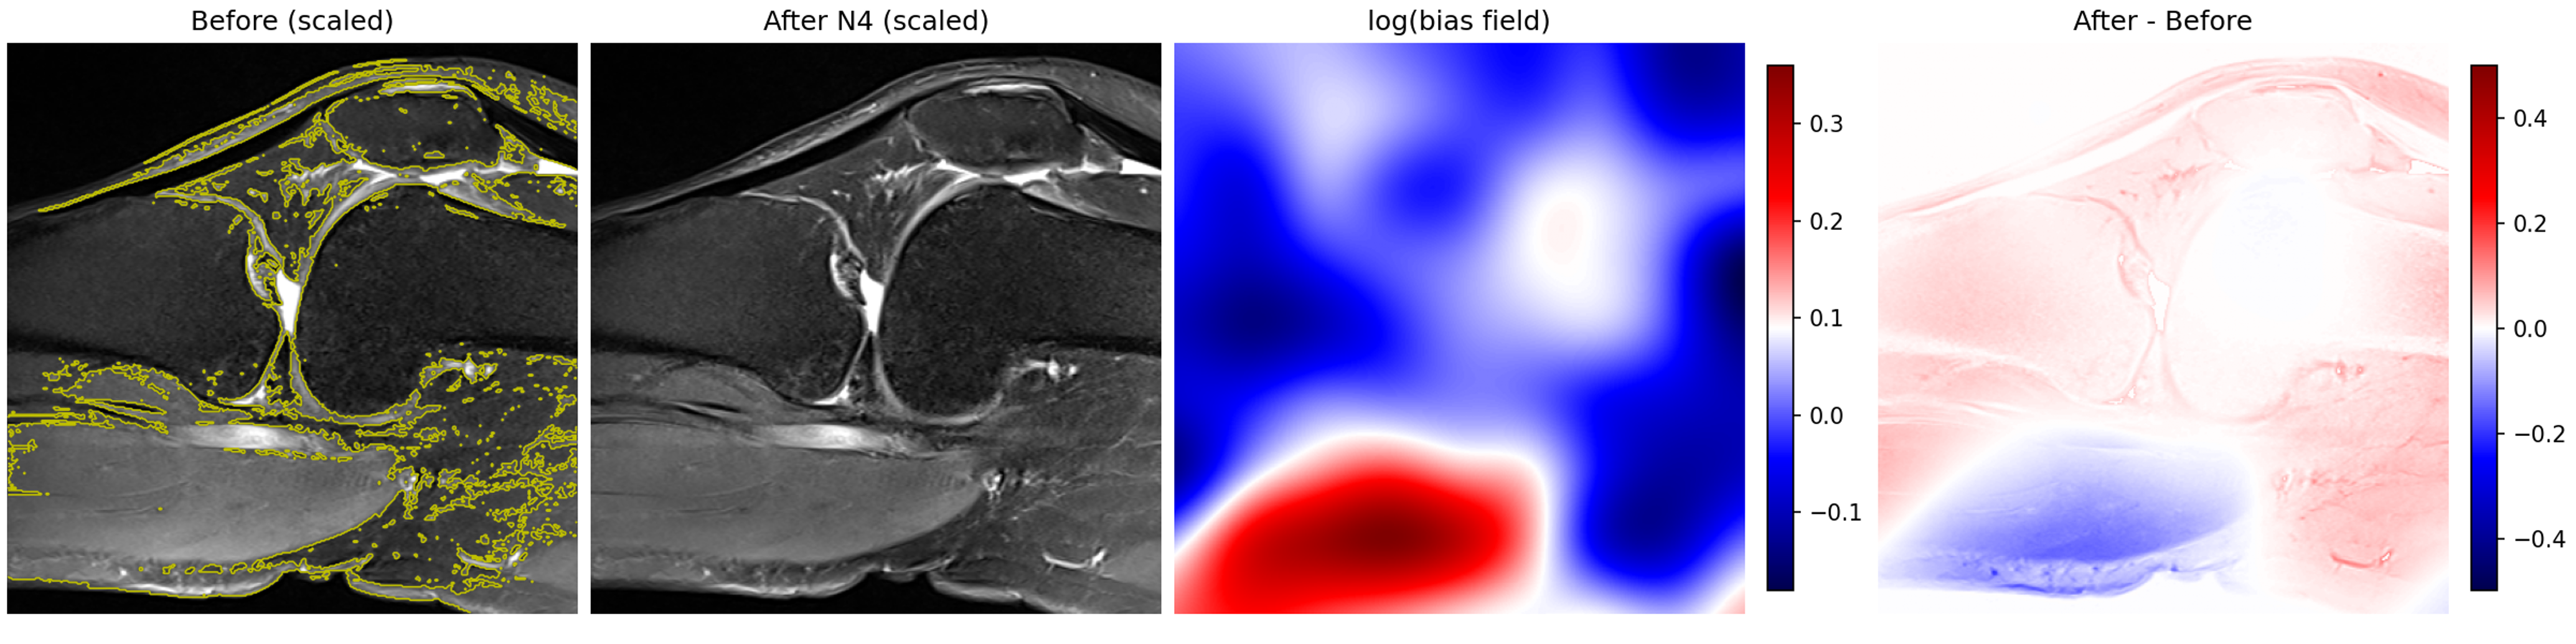
\includegraphics[width=1.0\linewidth]{figures/n4_correction.png}
        \caption{N4偏置场校正示例}
        \label{fig:n4_correction}
      \end{figure}
  \subsection{基于分辨率的空间重采样与 3D 全局归一化}
    在完成了 DICOM 到 NIfTI 的格式转换以及 N4 偏置场校正后，虽然单例 MRI 图像的内部低频伪影已被消除，
    但由于 500 例孤立 ACL 撕裂和 165 例多发韧带损伤（MLKI）患者的影像来源于真实的临床扫描环境，
    不同患者或不同批次之间在物理分辨率（Voxel Spacing）和绝对灰度分布上仍存在巨大的异质性。
    为了满足基于 ResNet-34 骨干网络的深度学习模型对统一张量输入的要求，并缩小与源域（OAI-ZIB 数据集）的底层特征鸿沟，
    本研究实施了严格的物理空间重采样与 3D 全局灰度归一化处理。
    \subsubsection{物理空间域的重采样（Resampling）与尺寸对齐}
      在卷积神经网络（CNN）中，特定大小的卷积核（如 3×3）在不同物理分辨率的图像上所涵盖的真实解剖学视野（即感受野，Receptive Field）是完全不同的。
      如果直接将原始尺度不一的临床 FSE 序列输入网络，会导致模型难以学习到软骨和骨骼的一致性几何形态特征。
      \par 为了消除这种尺度偏移，本研究在三维空间中对所有目标域数据进行了基于固定物理间距的全局重采样。
      考虑到 UDA 任务中需要将临床 FSE 影像与 OAI-ZIB 的 DESS 影像进行特征级对齐，
      本研究将目标分辨率强制映射到与源域一致的 \qty{0.36}{\milli\metre} $\times$ \qty{0.36}{\milli\metre} $\times$ \qty{0.7}{\milli\metre} 标准间距上。
      在重采样算法的选择上，采用了三线性插值（Trilinear Interpolation）以平滑地过渡体素值，避免近邻插值带来的阶梯状边缘伪影。
      \par 在物理分辨率统一后，各个样本的三维矩阵维度（Matrix Size）出现了长短不一的情况。
      为满足网络批处理（Batch Processing）的张量维度对齐要求，本研究进一步采用了中心裁剪（Center Crop）与边缘零填充（Zero-padding）相结合的策略，
      将每一张二维切片（Slice）的尺寸精准裁剪或填充至 384×384 像素。这一步骤在不破坏解剖结构比例的前提下，构建了与源域完全同构的输入空间。
      \subsubsection{图像特征域的 3D 全局归一化}
        由于MRI 的信号强度是相对的，其绝对灰度值高度依赖于扫描仪的硬件配置（如 1.5T 与 3.0T 磁体差异）和接收线圈的增益设置。
        如果不进行处理，这种全局亮度和对比度的巨大类间方差将主导网络的损失梯度，使其无法关注到微小的软骨边界或骨髓病变（BML）纹理。
        \par 在深度学习医学图像预处理中，常用的归一化方法包括最大最小值归一化（Min-Max Normalization）和 Z-score 归一化（Standardization）。
        本研究果断弃用了 Min-Max 归一化，因为该方法对图像中的极端异常值（Outliers，如由于血管流空效应或扫描仪伪影产生的极亮噪点）极度敏感，容易导致正常软组织的灰度被过度压缩。
        \par 本研究对所有重建后的三维体积应用了稳健的 Z-score 全局归一化策略。
        具体而言，算法首先通过阈值法剔除纯黑背景体素，随后在整个 3D 前景体积（Foreground Volume）内计算所有有效体素的灰度均值（$\mu$）和标准差（$\sigma$）。对于任意体素 $x$，其归一化后的值 $z$ 的计算公式为：
        \begin{equation}
          z = \frac{x - \mu}{\sigma}
        \end{equation}
        \par 该操作将每一例患者的 MRI 强度分布强制拉伸至均值为 0、标准差为 1 的标准正态分布区间内。
        这一极其关键的处理不仅消除了不同机器间的“对比度风格”壁垒，稳定了模型前向传播中的激活值分布，
        而且在后续利用阈值法或生成式模型提取 BML 时，使得原本微弱的水肿高信号在统计学分布上得以显著放大并更易于被网络捕获。
        \par 经过上述 DICOM 转换、N4 偏置场校正、空间重采样以及 Z-score 归一化处理，本研究成功将 665 例规格杂乱的临床多维数据转化为了结构高度统一的高质量特征张量。
        这为第四章改进型 DANN 网络进行跨域特征博弈与精准分割提供了极其纯净的数据基石。




